\chapter{Influence de la source}

Dans le processus d'auralisation, la prise de réponse impulsionnelle ou le calcul de celle ci est un passage important.

En réalité, la qualité du signal final dépend grandement de la qualité de la RI.

\section{Qualité d'une RI} % {{{1

L'estimation de la qualité d'une RI passe notamment par 3 facteurs :

\begin{itemize}
	\item la netteté de l'attaque ;
	\item un bon rapport signal/bruit (RSB) ; 
	\item la qualité de l'impulsion.
\end{itemize}

La netteté de l'attaque et la qualité de l'impulsion sont liées en fait, mais une impulsion bien générée sera toujours
tributaire de la qualité de la source, en cela, cette dernière est clairement le facteur limitant.

Un bon RSB est parfois assez difficile à obtenir (milieu bruyant, parasites, etc...), il peut toutefois être amélioré.

\subsection{Amélioration de la qualité de la RI} % {{{2

Plusieurs techniques peuvent permettre d'améliorer les différents paramètres d'une RI. On peut d'ailleurs regrouper ces
techniques en deux ensembles : celles agissant sur le procédé de mesure lui-même et celles agissant \textit{a
posteriori}. 

La second classe comporte de nombreuses techniques de traitement du signal et de réduction du bruit :

\begin{itemize}
    \item déconvolution de signaux ;
    \item filtrage simple ;
    \item filtrage Wiener.
\end{itemize}

Pour ce qui est des techniques interférant dans le procédé de mesure, on peut notamment citer la prise de réponses
fréquentielles plutôt qu'impulsionnelles ou l'utilisation de signaux MLS et de systèmes spécialisés (système CLIO\textsuperscript{\textsc{TM}} par
exemple).

La prise de réponses fréquentielles permet d'utiliser des enceintes avec de multiples hauts parleurs, même si ceux ci
n'ont pas des temps de réponse comparables. En effet, il s'agit d'émettre un bruit le plus large bande possible et de
calculer la fonction de tranfert dans le domaine fréquentiel :

$$H(F) = \frac{S(F)}{E(F)}$$

où $H(F)$ est la fonction de transfert en fréquentiel, $E(F)$ le signal excitateur et $S(F)$ le signal mesuré dans la
salle.

On peut ensuite repasser dans le domaine temporel pour récupérer une réponse impulsionnelle en appliquant une transformée
de Fourier inverse sur $H(F)$.

Les deux avantages de l'utilisation de réponses fréquentielles c'est qu'elles sont moyennables (ce qui permet de réduire
les erreurs) et qu'il est possible de les mesurer à fort niveau, améliorant ainsi le RSB. Il faut toutefois faire
attention à ce que toutes les fréquences soient excitées de manière semblable (là encore, les transducteurs sont
limitants).

La deuxième possibilité, impliquant des systèmes spécialisés, permet de mesurer des RI de bonne qualité même dans des
environnements (relativement) bruyants. C'est un avantage considérable de l'utilisation de signaux MLS (\textit{Maximum
Length Sequence}). Le système CLIO\textsuperscript{\textsc{TM}} permet ce genre de choses mais comme tout système
spécialisé, il demande un certain temps de prise en main. Il n'a pas été utilisé au cours de ce projet.

\section{Influence du ballon de baudruche} % {{{1

La réponse impulsionnelle d'une salle doit la caractériser et particulièrement les différentes réflexions induites
par sa géométrie.

Afin d'avoir une mesure la plus fidèle possible à la réalité du terrain, il faut que la source utilisée pour générer
l'impulsion (ou le bruit permettant la prise d'une réponse en fréquences) soit la plus omni-directionnelle possible.

L'utilisation d'un ballon de baudruche posait le souci que sa directivité est inconnue. Avec plus de temps, une
caractérisation de la directivité du ballon aurait pû être intéressante.

Une telle étude semble être en cours ou avoir été réalisée au LIMSI~\cite{Bru10}, malheureusement l'étude n'est pas
disponible à la consultation : pour ce projet, le ballon de baudruche sera donc considéré omnidirectionnel.

Le second incovénient soulevé par l'utilisation d'un ballon de baudruche est que la bande passante du son généré par
son éclatement n'est pas connue. Un éclatement de ballon de baudruche est donc mesuré en salle semi-anéchoïque (le
spectre est visible en figure~\ref{spk_ballon_anecho}).

\begin{figure}[h!]
\centering{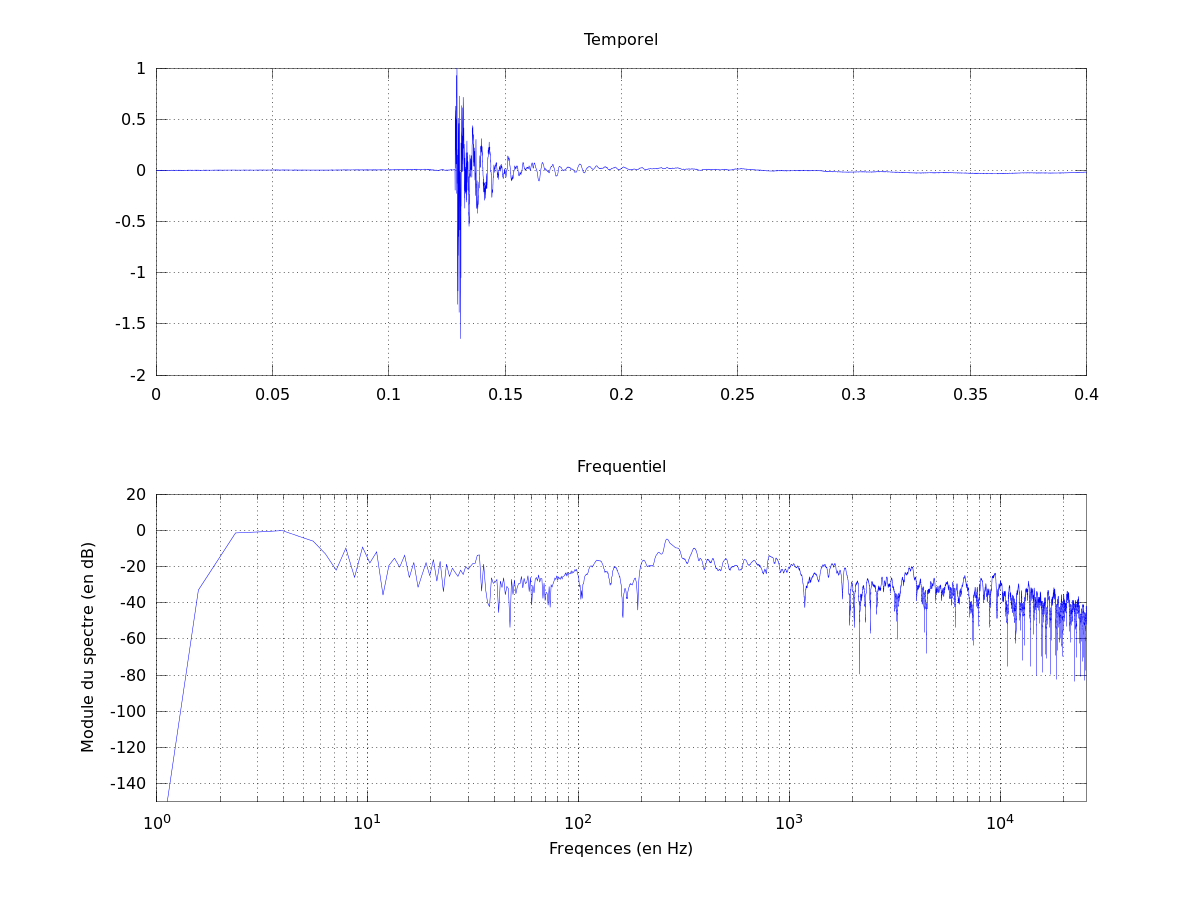
\includegraphics[width=10cm]{rep_ballon_anecho.png}}
\caption{\label{spk_ballon_anecho}Enregistrement temporel de l'éclatement d'un ballon de baudruche en salle
semi-anéchoïque (noter les réflexions visibles en temporel) et spectre en dB du signal.}
\end{figure}

La réponse en fréquence n'est donc clairement pas plate. On note une décroissance de 20dB par décade et une série de
minima en hautes fréquences ainsi qu'un creux dans la bande 10 - 200Hz.

\begin{figure}[h!]
\centering{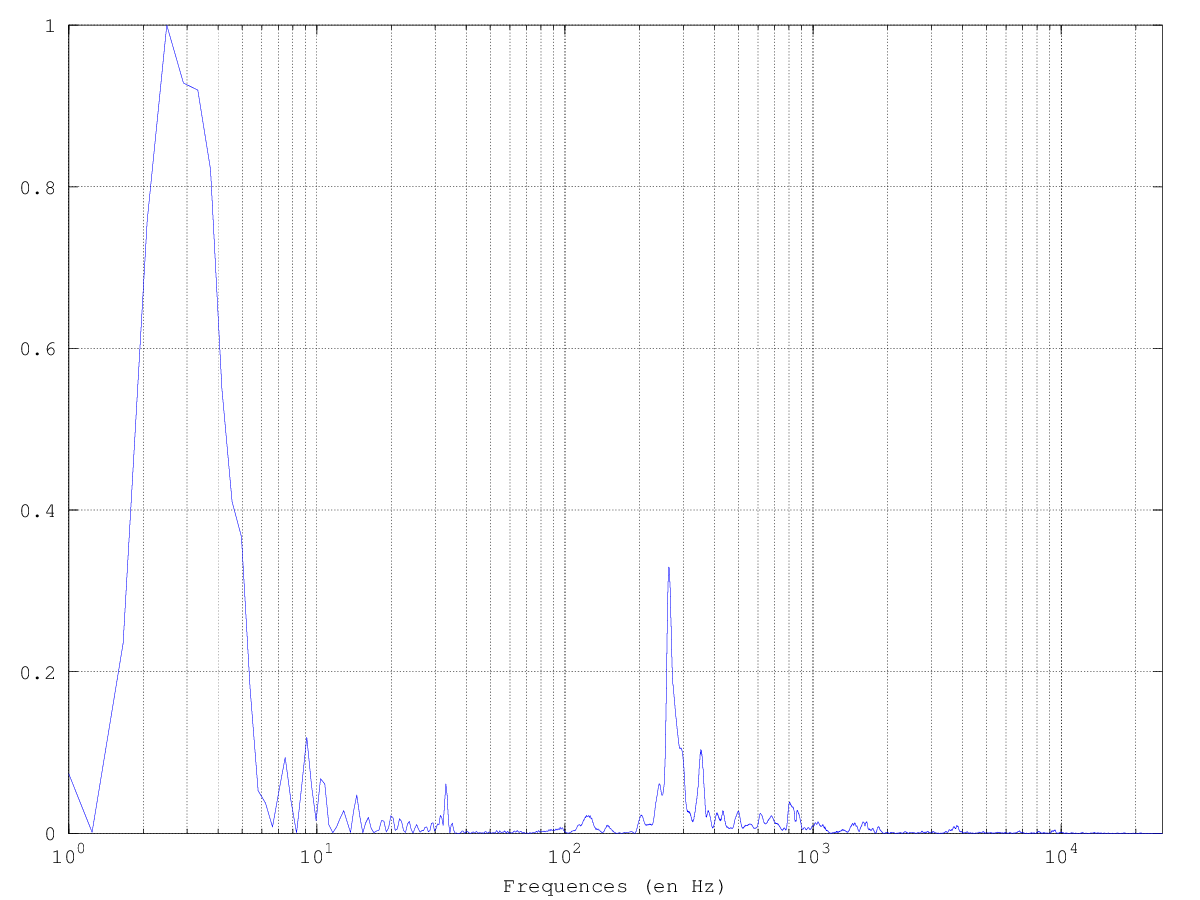
\includegraphics[width=10cm]{ballon_energie.png}}
\caption{\label{ballon_energie}Spectre d'énergie d'un ballon de baudruche en salle semi-anéchoïque.}
\end{figure}

Pour mieux saisir la correspondance entre la bande passante du ballon et les résultats à l'écoute, on observe le graphe
de la valeur absolue au carré du spectre. Cela nous donne le spectre d'énergie présenté en figure~\ref{ballon_energie}.

On remarque que l'énergie se situe principalement dans les basses fréquences (en deçà de 100Hz) et que 2 pics viennent
potentiellement perturber la RI entre 200 et 400Hz.

\section{Compensation de la source} % {{{1

Les sources utilisées ne sont donc pas parfaites, cependant il est possible de les prendre en considération lors du calcul du son convolué.
En effet, les imperfections dues à la chaîne d'excitation peuvent être modélisées par un filtre qui viendrait «avant» la salle modélisée par un système linéaire. De plus la chaîne d'acquisition est elle supposée parfaite ; en pratique ce n'est pas tout à fait le cas, mais devant l'imperfection de la chaine d'excitation l'approximation est correcte. Cette configuration est représentée sur le schéma figure~\ref{compensation}.
\begin{figure}[h!]
\centering{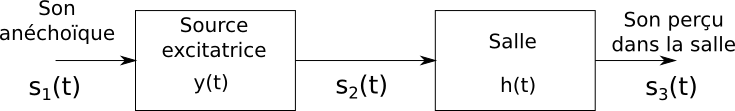
\includegraphics[width=10cm]{g4322.png}}
\caption{\label{compensation}Schéma du système étudié avec prise en compte de la chaîne d'excitation}
\end{figure}
Afin de pouvoir compenser la chaine d'excitation ; il faut donc déterminer $y(t)$. Cette grandeur correspond, dans le
cas du ballon, à la fonction permettant de passer d'une impulsion parfaite à celle donnée par le ballon : il s'agit de
la fonction de transfert du ballon. En définitif, pour connaître cette fonction de transfert, une mesure de l'éclatement d'un ballon en salle anéchoïque (là où la salle a le moins d'influence) est réalisée. Cette mesure est présentée en figure~\ref{spk_ballon_anecho}.
Une fois $y(t)$ determiné, il ne reste qu'à en déduire $h(t)$.
On sait que :
\begin{eqnarray*}
s_1 (t) \ast y(t) = s_2 (t) \Leftrightarrow S_1 (F) \times Y(F) = S_2 (F)\\
s_2 (t) \ast h (t) = s_3 (t) \Leftrightarrow S_2 (F) \times H(F) = S_3 (F)
\end{eqnarray*}
On peut donc en déduire que :
\begin{eqnarray*}
h(t) = \mathcal{F}^{-1}\left\{ \frac{S_3 (F)}{S_2(F)}\right\} 
\end{eqnarray*}
Bien que retrouver la réponse impulsionnelle de la salle exempte de l'influence du ballon semble simple sur un plan
théorique, d'un point de vue pratique, de grosses difficultés ont été rencontrées. En effet, voici en
figure~\ref{bizarre} la réponse impulsionnelle obtenue dans le domaine temporel et fréquentiel : 

\begin{figure}[h!]
\centering{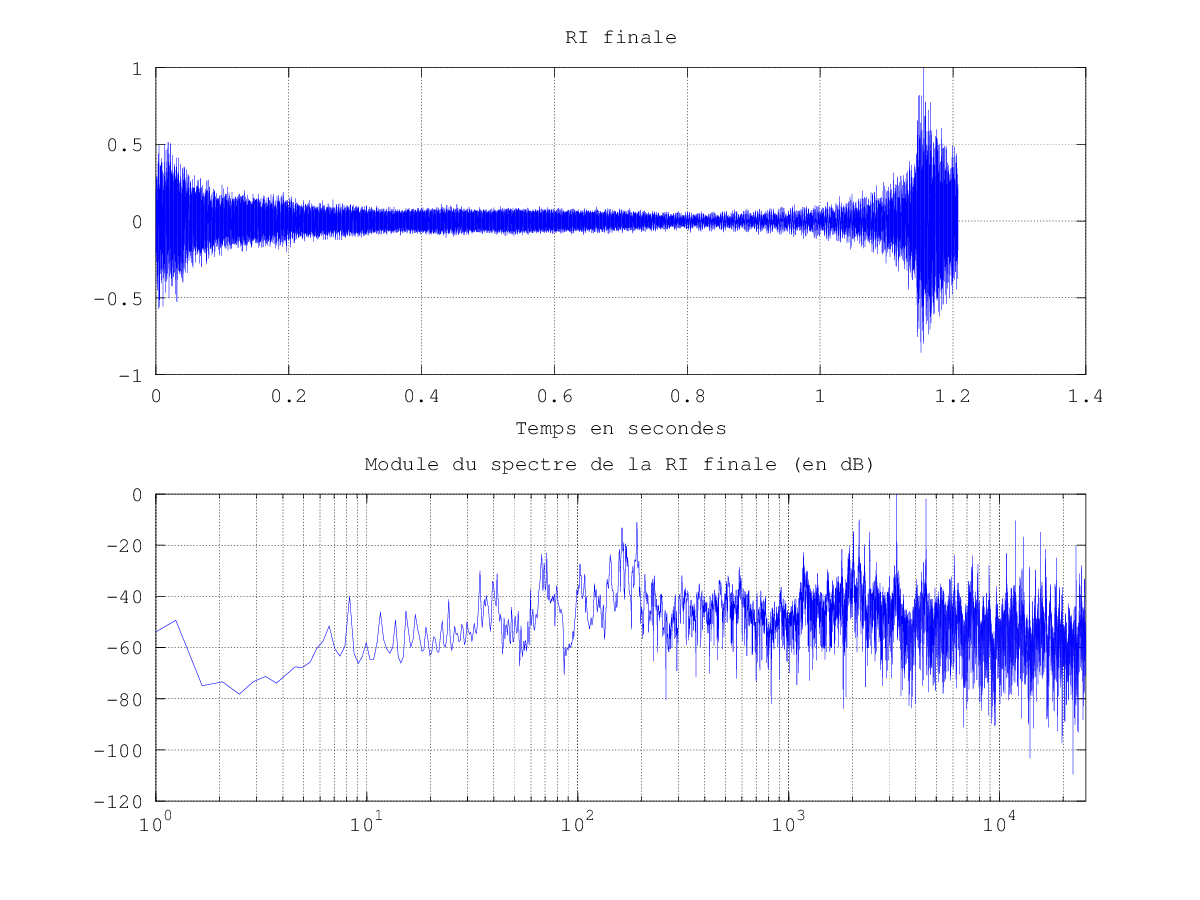
\includegraphics[width=10cm]{spk_compensation.png}}
\caption{\label{bizarre}Réponse impulsionnelle calculée représentée temporellement et fréquentiellement.}
\end{figure}
Le résultat ne semble donc pas concluant. Il est probable que le problème vienne des modifications éventuelles
qu'apportent la transformée de Fourier au niveau de la phase des signaux. Cependant nos connaissances sur le sujet sont
trop limitées pour permettre de se pencher de manière approfondie sur la question.

